\documentclass[10pt,landscape]{article}
\usepackage[letterpaper,landscape,margin=0.16in]{geometry}
\usepackage{amsmath,amssymb,mathtools,array,booktabs}
\usepackage{graphicx}
\usepackage[most]{tcolorbox}
\usepackage{xcolor,microtype,enumitem}
\pagestyle{empty}
\setlength{\parindent}{0pt}
\setlength{\parskip}{0pt}
\setlength{\tabcolsep}{1.25pt}
\renewcommand{\arraystretch}{0.93}
\setlength{\abovedisplayskip}{0.25pt}
\setlength{\belowdisplayskip}{0.25pt}
\setlength{\abovedisplayshortskip}{0.1pt}
\setlength{\belowdisplayshortskip}{0.1pt}
\setlist{nosep,leftmargin=9pt}
\hyphenpenalty=10000
\exhyphenpenalty=10000
\pretolerance=4000
\tolerance=5000
\emergencystretch=2em
\color{black}

\newcommand{\R}{\mathbb{R}}
\newcommand{\teach}{\textbf{PROFESSOR TEACHES - THEORY}\quad}
\newcommand{\recognize}{\textbf{HOW TO RECOGNIZE}\quad}
\newcommand{\procedure}{\textbf{HOW TO SOLVE}\quad}
\newcommand{\question}{\textbf{MOCK / HOMEWORK QUESTION}\quad}
\newcommand{\example}{\textbf{STUDENT APPLICATION - WHAT TO WRITE}\quad}
\newcommand{\verify}{\textbf{VERIFY}\quad}
\newcommand{\stuck}{\textbf{IF STUCK}\quad}

\newtcolorbox{blk}[1]{
  colback=white,colframe=black,coltitle=white,colbacktitle=black,
  boxrule=.55pt,arc=.25pt,left=2pt,right=2pt,top=.8pt,bottom=.8pt,
  title=\textbf{#1},fonttitle=\bfseries,before skip=.3pt,after skip=.3pt
}
\newtcolorbox{theorybox}[1]{
  colback=white,colframe=black,boxrule=.45pt,arc=.2pt,
  left=2pt,right=2pt,top=1.1pt,bottom=1.1pt,
  title=\textbf{#1},coltitle=black,colbacktitle=white,
  fonttitle=\bfseries,before skip=0pt,after skip=0pt
}

\begin{document}

% =============================================================
% PAGE 1
% =============================================================
\fontsize{5.65}{5.95}\selectfont
\begin{center}
{\fontsize{10.4}{10.7}\selectfont\bfseries IEE 574 EXAM 1 - COURSE THEORY $\rightarrow$ RECOGNIZE $\rightarrow$ SOLVE $\rightarrow$ APPLY}\\[-1pt]
{\fontsize{5.9}{6.1}\selectfont Courses 1--6 theory is explicit; mock/homework problems are student applications. The four graduated-paper images are inserted unchanged and only uniformly scaled.}
\end{center}\vspace{-1.5pt}

% ---------- PAGE 1 THEORY BAND: COURSES 1--4 ----------
{\fontsize{5.25}{5.50}\selectfont
\noindent
\begin{minipage}[t]{0.245\textwidth}\vspace{0pt}
\begin{theorybox}{COURSE 1 - OPERATIONS RESEARCH}
\teach Scientific method for decision-making and optimization under constraints.
\[
\boxed{\begin{gathered}
\text{define problem/data}\to\text{formulate model}\\[-1pt]
\to\text{solve}\to\text{analyze}
\end{gathered}}
\]
Ask: \textbf{what is given? what is chosen? what rules must hold? what is optimized?}
\end{theorybox}
\end{minipage}\hfill
\begin{minipage}[t]{0.245\textwidth}\vspace{0pt}
\begin{theorybox}{COURSE 2 - BASIC LINEAR ALGEBRA}
\[
\boxed{a^\top b=0\Rightarrow a\perp b}
\]
\[
\boxed{\sum_j\lambda_j a_j=0\Rightarrow\lambda_j=0\ \forall j}
\]
This is linear independence. $\operatorname{Span}(a_1,\ldots,a_k)$ = all linear combinations.
\[
\boxed{\text{Basis}=\text{linearly independent vectors that span the space}}
\]
\end{theorybox}
\end{minipage}\hfill
\begin{minipage}[t]{0.245\textwidth}\vspace{0pt}
\begin{theorybox}{COURSE 3 - MATHEMATICAL MODELING}
\[
\boxed{\begin{gathered}
\text{Input Data}+\text{Decision Variables}\\[-1pt]
+\text{Constraints}+\text{Objective Function}
\end{gathered}}
\]
Parameter = known input; Decision Variable = quantity chosen. Every index is summed over or explicitly quantified. \textbf{No dangling subscripts.}
\[
\boxed{\begin{gathered}
\text{indices}\to\text{parameters}\to\text{variables}\\[-1pt]
\to\text{objective}\to\text{constraints}\to\text{domain}
\end{gathered}}
\]
\end{theorybox}
\end{minipage}\hfill
\begin{minipage}[t]{0.245\textwidth}\vspace{0pt}
\begin{theorybox}{COURSE 4 - STANDARD FORM}
\[
\boxed{\min c^\top x\quad\text{s.t. }Ax=b,\ x\ge0}
\]
\[
x\le0\Rightarrow x=-x',\ x'\ge0;\qquad x\in\R\Rightarrow x=x^+-x^-.
\]
\[
\le\Rightarrow+s,\qquad \ge\Rightarrow-s,\qquad \max c^\top x\Rightarrow\min(-c^\top x).
\]
\[
\boxed{\min|f(x)|\Rightarrow\min t:\ t\ge f(x),\ t\ge-f(x)}
\]
\end{theorybox}
\end{minipage}}
\vspace{1.2pt}
% ---------- PAGE 1 APPLICATION BAND: 3 COLUMNS ----------
\noindent
\begin{minipage}[t]{0.327\textwidth}\vspace{0pt}
\begin{blk}{PROBLEM 1 - RESOURCE ALLOCATION / BLENDING}
\recognize products/blends + profit + limited resources $\Rightarrow$ one Decision Variable per product and one constraint per limited resource.

\procedure Let $i\in I$ index resources, $j\in J$ products:
\[
\begin{aligned}
a_{ij}&=\text{resource }i\text{ used per unit of }j,\\
b_i&=\text{available resource }i,\qquad p_j=\text{profit/unit of }j.
\end{aligned}
\]
\[
\boxed{\begin{aligned}
\max\quad&\sum_{j\in J}p_jx_j\\
\text{s.t.}\quad&\sum_{j\in J}a_{ij}x_j\le b_i\ \forall i,\qquad x_j\ge0\ \forall j.
\end{aligned}}
\]

\question Four blends use three limited stocks. Formulate the Linear Programming model.

\example
\textbf{1. Sets:} $I=\{1,2,3\}$ stocks; $J=\{1,2,3,4\}$ blends.

\textbf{2. Parameters:}
\[
\begin{aligned}
a_{ij}&=\text{fraction of stock }i\text{ in one gallon of blend }j,\\
b_i&=\text{available gallons of stock }i,\qquad p_j=\text{profit per gallon of blend }j.
\end{aligned}
\]
\[
A=\begin{bmatrix}.40&.20&.50&.20\\.20&.20&.05&.40\\.40&.60&.45&.40\end{bmatrix},\quad
b=\begin{bmatrix}15000\\14000\\20000\end{bmatrix},\quad p=\begin{bmatrix}.10\\.11\\.14\\.25\end{bmatrix}.
\]
\textbf{3. Decision Variable:}
\[
\boxed{x_j=\text{gallons of blend }j\text{ produced},\quad j\in J}.
\]
\textbf{4. Objective Function:}
\[
\boxed{\max\ .10x_1+.11x_2+.14x_3+.25x_4}.
\]
\textbf{5. Constraints:}
\[
\begin{aligned}
.40x_1+.20x_2+.50x_3+.20x_4&\le15000,\\
.20x_1+.20x_2+.05x_3+.40x_4&\le14000,\\
.40x_1+.60x_2+.45x_3+.40x_4&\le20000,\\
x_1,x_2,x_3,x_4&\ge0.
\end{aligned}
\]
\textbf{6. Final model:}
\[
{\fontsize{5.0}{5.15}\selectfont
\boxed{\begin{aligned}
\max\quad&.10x_1+.11x_2+.14x_3+.25x_4\\
\text{s.t.}\quad&.40x_1+.20x_2+.50x_3+.20x_4\le15000,\\
&.20x_1+.20x_2+.05x_3+.40x_4\le14000,\\
&.40x_1+.60x_2+.45x_3+.40x_4\le20000,\\
&x_1,x_2,x_3,x_4\ge0.
\end{aligned}}}
\]
\stuck What do I choose? $\Rightarrow x_j$. What is limited? $\Rightarrow$ one constraint for each $i$.
\end{blk}
\end{minipage}\hfill
%
\begin{minipage}[t]{0.327\textwidth}\vspace{0pt}
\begin{blk}{PROBLEM 2 - TRANSPORTATION}
\recognize from-to / shipping / source-destination $\Rightarrow x_{ij}$; if a route does not exist, do not create that Decision Variable.

\procedure $I=$ sources, $J=$ destinations, $\mathcal R\subseteq I\times J=$ allowed routes:
\[
\boxed{\begin{aligned}
\min\quad&\sum_{(i,j)\in\mathcal R}c_{ij}x_{ij}\\
\text{s.t.}\quad&\sum_{j:(i,j)\in\mathcal R}x_{ij}\le a_i\ \forall i,\\
&\sum_{i:(i,j)\in\mathcal R}x_{ij}\ge d_j\ \forall j,\\
&x_{ij}\ge0,\ (i,j)\in\mathcal R.
\end{aligned}}
\]
\begin{center}
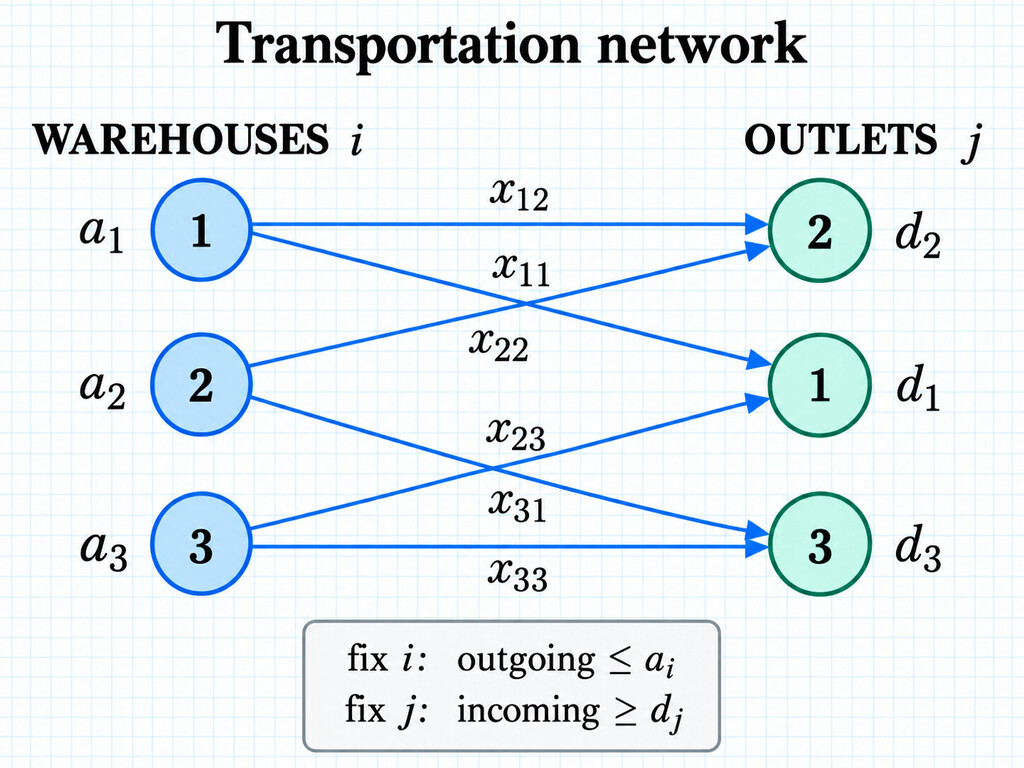
\includegraphics[height=2.30cm,keepaspectratio]{figures/transportation_network.jpg}
\end{center}
\textbf{Image rule:} fix $i$ $\Rightarrow$ sum outgoing routes; fix $j$ $\Rightarrow$ sum incoming routes.

\question Routes $T_{11},T_{12},T_{22},T_{23},T_{31},T_{33}$; cost $10$; supplies $(4,6,8)$; demands $(8,3,7)$.

\example
\textbf{1. Sets/routes:}
\[
I=J=\{1,2,3\},\qquad\mathcal R=\{(1,1),(1,2),(2,2),(2,3),(3,1),(3,3)\}.
\]
\textbf{2. Parameters/variables:}
\[
a=(4,6,8),\quad d=(8,3,7),\quad c_{ij}=10,
\]
\[
\boxed{x_{ij}=\text{units shipped from warehouse }i\text{ to outlet }j}.
\]
\textbf{3. Objective:}
\[
\boxed{\min\ 10(x_{11}+x_{12}+x_{22}+x_{23}+x_{31}+x_{33})}.
\]
\textbf{4. Supply:} $x_{11}+x_{12}\le4$, $x_{22}+x_{23}\le6$, $x_{31}+x_{33}\le8$.

\textbf{5. Demand:} $x_{11}+x_{31}\ge8$, $x_{12}+x_{22}\ge3$, $x_{23}+x_{33}\ge7$.

\textbf{6. Domain:} $x_{11},x_{12},x_{22},x_{23},x_{31},x_{33}\ge0$.

\textbf{7. Final model:}
\[
{\fontsize{4.9}{5.08}\selectfont
\boxed{\begin{aligned}
\min\quad&10(x_{11}+x_{12}+x_{22}+x_{23}+x_{31}+x_{33})\\
\text{s.t.}\quad&x_{11}+x_{12}\le4,\ x_{22}+x_{23}\le6,\ x_{31}+x_{33}\le8,\\
&x_{11}+x_{31}\ge8,\ x_{12}+x_{22}\ge3,\ x_{23}+x_{33}\ge7,\\
&x_{11},x_{12},x_{22},x_{23},x_{31},x_{33}\ge0.
\end{aligned}}}
\]
\verify $\sum_i a_i=\sum_jd_j=18$; every feasible plan ships $18$ units and, since every route costs $10$, has total cost $180$.
\end{blk}
\end{minipage}\hfill
%
\begin{minipage}[t]{0.327\textwidth}\vspace{0pt}
\begin{blk}{PROBLEM 3 - STANDARD FORM + TRUE/FALSE}
\recognize variable-sign restrictions, inequalities, maximization, or absolute values $\Rightarrow$ normalize to $\min c^\top x$ s.t. $Ax=b$, $x\ge0$.

\procedure
\[
\boxed{\begin{gathered}
\text{fix signs}\to\text{equalities}\to\text{minimization}\\[-1pt]
\to\text{freeze }x\to\text{read }A,b,c
\end{gathered}}
\]
Always preserve $x_j\leftrightarrow A_j\leftrightarrow c_j$.

\question Convert $\min|x_1+x_4|$ with $x_1-x_2\ge1$, $x_3+x_4\le3$, $x_1,x_2\ge0$, $x_3\le0$, $x_4\in\R$ to Standard Form.

\example
\textbf{1. Signs:}
\[
x_3=-\bar x_3,\quad x_4=x_4^+-x_4^-,\qquad \bar x_3,x_4^+,x_4^-\ge0.
\]
\textbf{2. Absolute value:} introduce $t\ge0$ and minimize $t$:
\[
t\ge x_1+x_4^+-x_4^-,\qquad t\ge-x_1-x_4^++x_4^-.
\]
\textbf{3. Equalities:} $s_1,s_2,s_3,s_4\ge0$,
\[
\begin{aligned}
x_1-x_2-s_1&=1,\\
-\bar x_3+x_4^+-x_4^-+s_2&=3,\\
x_1+x_4^+-x_4^- -t+s_3&=0,\\
-x_1-x_4^++x_4^- -t+s_4&=0.
\end{aligned}
\]
\textbf{4. Variable order:}
\[
\boxed{x=(x_1,x_2,\bar x_3,x_4^+,x_4^-,t,s_1,s_2,s_3,s_4)^\top\ge0}.
\]
\textbf{5. Read off $A,b,c$:}
\[
{\fontsize{4.85}{5.0}\selectfont
A=\begin{bmatrix}
1&-1&0&0&0&0&-1&0&0&0\\
0&0&-1&1&-1&0&0&1&0&0\\
1&0&0&1&-1&-1&0&0&1&0\\
-1&0&0&-1&1&-1&0&0&0&1
\end{bmatrix}}
\]
\[
b=(1,3,0,0)^\top,\qquad c=(0,0,0,0,0,1,0,0,0,0)^\top.
\]
Audit: $A\in\R^{4\times10}$, $x,c\in\R^{10}$, $b\in\R^4$.

\textbf{6. True/False:}
\[
\boxed{(a)\ T\qquad(b)\ T\qquad(c)\ T\qquad(d)\ F}.
\]
Optimal $\Rightarrow$ feasible; Standard Form feasibility includes $x\ge0$; for minimization the improving direction is $-c$.
\end{blk}
\end{minipage}

\newpage

% =============================================================
% PAGE 2
% =============================================================
\fontsize{5.55}{5.85}\selectfont
\begin{center}
{\fontsize{10.2}{10.5}\selectfont\bfseries IEE 574 EXAM 1 - GEOMETRY, GRAPHICAL METHOD, BASIC SOLUTIONS}\\[-1pt]
{\fontsize{5.85}{6.05}\selectfont Course 5 and Course 6 theory first; exact graduated-paper images below are unchanged and uniformly scaled.}
\end{center}\vspace{-1.5pt}

% ---------- PAGE 2 THEORY BAND: COURSES 5--6 ----------
{\fontsize{5.05}{5.28}\selectfont
\noindent
\begin{minipage}[t]{0.245\textwidth}\vspace{0pt}
\begin{theorybox}{COURSE 5A - FEASIBILITY / CONVEXITY}
Feasible solution satisfies all constraints. Optimal solution is feasible and has the best objective value.
\[
\boxed{\text{optimal}\Rightarrow\text{feasible}},\qquad\boxed{\text{feasible}\not\Rightarrow\text{optimal}}.
\]
Convex combination: $x=\sum_i\lambda_i x_i$, $\lambda_i\ge0$, $\sum_i\lambda_i=1$. Convex set: every line segment between two feasible points remains in the set.
\end{theorybox}
\end{minipage}\hfill
\begin{minipage}[t]{0.245\textwidth}\vspace{0pt}
\begin{theorybox}{COURSE 5B - HYPERPLANE / HALF-SPACE}
\[
\boxed{H=\{x:a^\top x=b\}},\qquad x^0\in H\Rightarrow\boxed{a^\top(x-x^0)=0}.
\]
$a$ is normal to $H$.
\[
\boxed{a^\top(x-x^0)=\|a\|\,\|x-x^0\|\cos\theta}.
\]
Acute $\theta\Rightarrow+$; $90^\circ\Rightarrow0$; obtuse $\Rightarrow-$. The sign determines the Half-Space.
\end{theorybox}
\end{minipage}\hfill
\begin{minipage}[t]{0.245\textwidth}\vspace{0pt}
\begin{theorybox}{COURSE 5C - POLYHEDRON / RECESSION}
\[
\boxed{\text{Polyhedron}=\text{intersection of Half-Spaces}}
\]
\[
\boxed{\text{Polytope}=\text{bounded Polyhedron}}.
\]
$d\ne0$ is a Recession Direction if $x+\lambda d\in X$ for all $x\in X$, $\lambda\ge0$. Bounded set $\Rightarrow$ no nonzero Recession Direction.
\[
\begin{gathered}
X=\{x:Ax\le b,x\ge0\}\Rightarrow Ad\le0,\ d\ge0,\\[-1pt]
Ax=b\Rightarrow Ad=0,\ d\ge0.
\end{gathered}
\]
Extreme Direction = recession direction not expressible as a strict conic combination of two distinct recession directions.
\end{theorybox}
\end{minipage}\hfill
\begin{minipage}[t]{0.245\textwidth}\vspace{0pt}
\begin{theorybox}{COURSE 6 - GRAPHICAL / BASIC SOLUTIONS}
Boundary: $a_1x_1+a_2x_2=b$. Objective contours: $c^\top x=z$.
\[
\boxed{\max\Rightarrow+c,\qquad\min\Rightarrow-c}.
\]
Finite optimum $\Rightarrow$ there exists an optimal Extreme Point.
\[
\boxed{\text{Extreme Point}\Longleftrightarrow\text{Basic Feasible Solution}}.
\]
Basic Solution: choose $m$ independent columns, set other $n-m$ variables to $0$, solve; feasible iff $x\ge0$.
\[
\boxed{\begin{gathered}
\text{unique optimum; infinitely many optima;}\\[-1pt]
\text{infeasible; unbounded}
\end{gathered}}
\]
Unbounded feasible region $\not\Rightarrow$ unbounded objective value.
\end{theorybox}
\end{minipage}}
\vspace{1.1pt}
% ---------- PAGE 2 APPLICATION BAND: 3 COLUMNS ----------
\noindent
\begin{minipage}[t]{0.315\textwidth}\vspace{0pt}
\begin{blk}{GEOMETRY APPLICATIONS - HOMEWORK 2}
\textbf{A. Hyperplane / Half-Spaces.}
\[
H:2x_1+x_2=4,\quad a=(2,1)^\top,\quad x^0=(1,2)^\top.
\]
\begin{center}
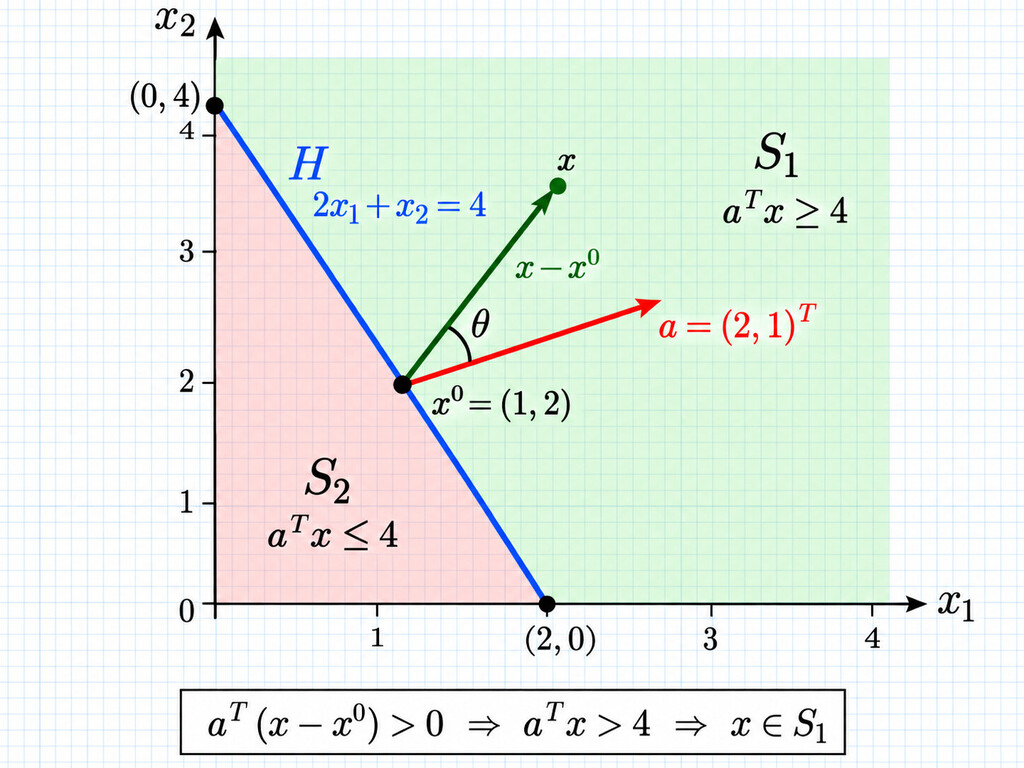
\includegraphics[height=2.75cm,keepaspectratio]{figures/hyperplane.jpg}
\end{center}
Acute angle between $x-x^0$ and $a$:
\[
\boxed{a^\top(x-x^0)>0\Rightarrow a^\top x>4\Rightarrow x\in S_1}.
\]

\textbf{B. Polyhedron / Recession Directions.}
\[
X=\{(x_1,x_2):x_1-2x_2\ge-6,\ x_1-x_2\ge-2,\ x_1\ge0,\ x_2\ge1\}.
\]
Equivalently $x_2\le\frac12x_1+3$, $x_2\le x_1+2$, $x_1\ge0$, $x_2\ge1$.
\begin{center}
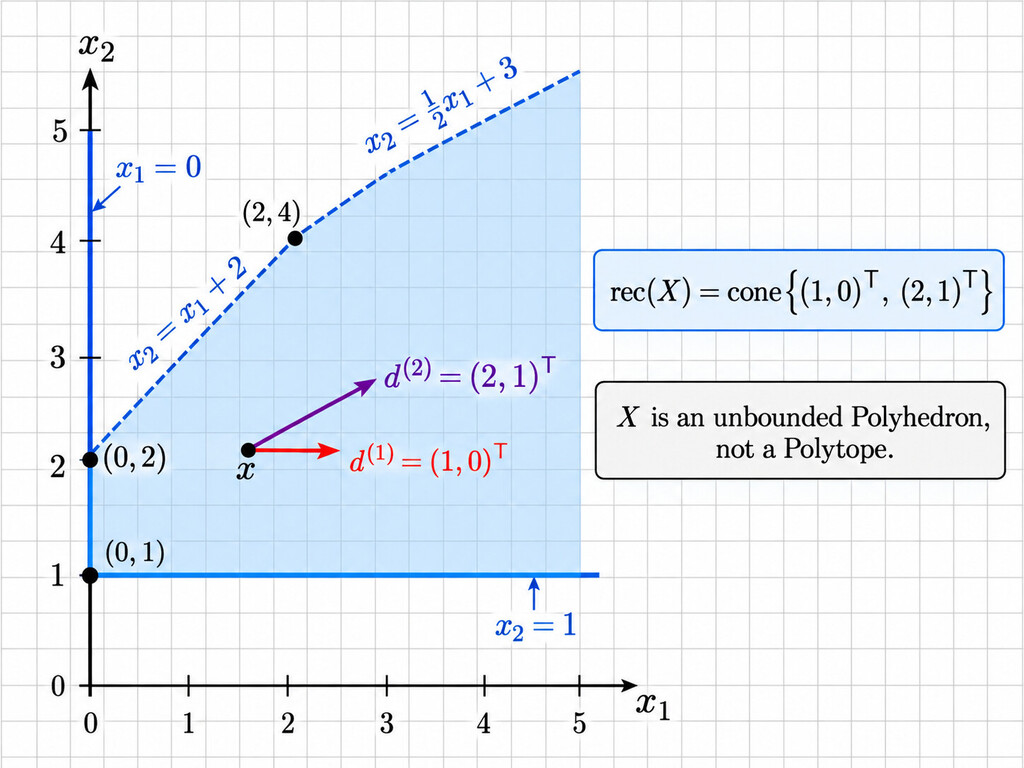
\includegraphics[height=2.75cm,keepaspectratio]{figures/recession_polyhedron.jpg}
\end{center}
Vertices: $\boxed{(0,1),(0,2),(2,4)}$. The set is unbounded, hence a Polyhedron but not a Polytope.
\[
\operatorname{rec}(X)=\{d:d_2\ge0,\ d_1\ge2d_2\}=\operatorname{cone}\{(1,0),(2,1)\}.
\]
\[
\boxed{d^{(1)}=(1,0)^\top,\qquad d^{(2)}=(2,1)^\top}.
\]
\end{blk}
\end{minipage}\hfill
%
\begin{minipage}[t]{0.345\textwidth}\vspace{0pt}
\begin{blk}{MOCK PROBLEM 4 - GRAPHICAL METHOD + OPTIMALITY}
\recognize two Decision Variables + linear inequalities + ``draw/contours/improving direction'' $\Rightarrow$ Graphical Method.

\procedure boundary lines $\to$ feasible Half-Spaces $\to$ Extreme Points $\to$ contours $c^\top x=z$ $\to$ improving direction $\to$ optimum.

\question
\[
\max\ 2x_1+5x_2\quad\text{s.t. }-x_1+2x_2\le16,\ 5x_1+3x_2\le50,\ x_2\le8,\ x_1,x_2\ge0.
\]

\example
\textbf{1. Boundaries:}
\[
C_1:-x_1+2x_2=16,\quad C_2:5x_1+3x_2=50,\quad C_3:x_2=8.
\]
\textbf{2. Redundancy:} because $x_1\ge0$, $x_2\le8$,
\[
-x_1+2x_2\le2x_2\le16\Rightarrow\boxed{C_1\text{ is redundant}}.
\]
\textbf{3. Extreme Points:}
\[
\begin{aligned}
x_2=0,\ C_2&\Rightarrow(10,0),\\
x_1=0,\ C_3&\Rightarrow(0,8),\\
x_2=8,\ C_2&\Rightarrow(26/5,8).
\end{aligned}
\]
$C_1\cap C_2=(4,10)$ is infeasible; include $(0,0)$.
\[
\boxed{(0,0),\ (10,0),\ (0,8),\ (26/5,8)}.
\]
\textbf{4. Objective geometry:}
\[
2x_1+5x_2=z,\quad c=(2,5)^\top,\quad\boxed{\text{improving direction}=+c}.
\]
\begin{center}
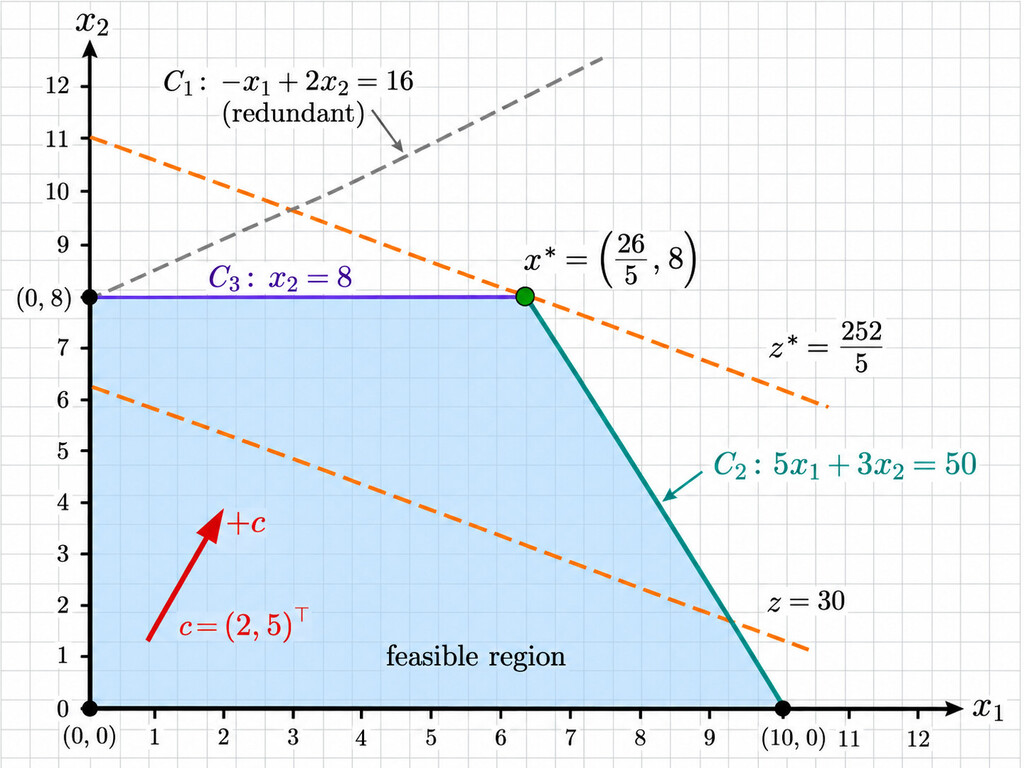
\includegraphics[height=2.95cm,keepaspectratio]{figures/graphical_lp.jpg}
\end{center}
\textbf{5. Evaluate Extreme Points:}
\[
\begin{array}{c|cccc}x&(0,0)&(10,0)&(0,8)&(26/5,8)\\\hline Z(x)&0&20&40&252/5\end{array}
\]
\[
\boxed{x^*=(26/5,8),\qquad z^*=252/5=50.4,\qquad X^*=\{(26/5,8)\}}.
\]
\end{blk}
\end{minipage}\hfill
%
\begin{minipage}[t]{0.330\textwidth}\vspace{0pt}
\begin{blk}{MOCK PROBLEM 4 - ALL BASIC SOLUTIONS}
\recognize ``find all Basic Solutions'' $\Rightarrow$ Standard Form, count $m,n$, enumerate candidate bases, solve, then test $x\ge0$.

\question Find all Basic Solutions and indicate which are Basic Feasible Solutions.

\example
\textbf{1. Standard Form:}
\[
\begin{aligned}
-x_1+2x_2+s_1&=16,\\
5x_1+3x_2+s_2&=50,\\
x_2+s_3&=8,
\end{aligned}
\qquad x_1,x_2,s_1,s_2,s_3\ge0.
\]
\[
A=\begin{bmatrix}-1&2&1&0&0\\5&3&0&1&0\\0&1&0&0&1\end{bmatrix},\qquad b=\begin{bmatrix}16\\50\\8\end{bmatrix}.
\]
$m=3$, $n=5$ $\Rightarrow\binom53=10$ candidate 3-column selections.

\textbf{2. Complete basis audit:}
\[
{\fontsize{4.55}{4.78}\selectfont
\begin{array}{c|l}
\text{Basic variables}&\text{solution / status}\\\hline
(x_1,x_2,s_1)&(26/5,8,26/5,0,0)\ \text{Basic Feasible}\\
(x_1,x_2,s_2)&(0,8,0,26,0)\ \text{Basic Feasible}\\
(x_1,x_2,s_3)&(4,10,0,0,-2)\ \text{infeasible}\\
(x_1,s_1,s_2)&\text{dependent; not a basis}\\
(x_1,s_1,s_3)&(10,0,26,0,8)\ \text{Basic Feasible}\\
(x_1,s_2,s_3)&(-16,0,0,130,8)\ \text{infeasible}\\
(x_2,s_1,s_2)&(0,8,0,26,0)\ \text{Basic Feasible}\\
(x_2,s_1,s_3)&(0,50/3,-52/3,0,-26/3)\ \text{infeasible}\\
(x_2,s_2,s_3)&(0,8,0,26,0)\ \text{Basic Feasible}\\
(s_1,s_2,s_3)&(0,0,16,50,8)\ \text{Basic Feasible}
\end{array}}
\]
\textbf{3. Distinct Basic Solutions:} seven distinct solution vectors occur; $(0,8,0,26,0)$ is generated by three bases.

\textbf{4. Basic Feasible Solutions:}
\[
\boxed{\begin{gathered}
(26/5,8,26/5,0,0),\ (0,8,0,26,0),\\
(10,0,26,0,8),\ (0,0,16,50,8).
\end{gathered}}
\]
Original $(x_1,x_2)$ space:
\[
\boxed{(26/5,8),\ (0,8),\ (10,0),\ (0,0)}.
\]
These are exactly the four Extreme Points.

\textbf{5. Degeneracy:} $(0,8,0,26,0)$ comes from bases $(x_1,x_2,s_2)$, $(x_2,s_1,s_2)$, $(x_2,s_2,s_3)$; hence $(0,8)$ is degenerate.
\end{blk}
\end{minipage}

\end{document}